
Depois de analisadas as caracteristicas das 3 ferramentas pré-selecionados, a escolhida foi o \textit{\textbf{GatherSpace}}.

Hoffmann (\citeyear{hoffmann03}) diz que um dos requisitos da ferramenta de gerenciamento de requisitos deve ser
a possibilidade de um acesso pela internet, o que tornará a instalação de uma aplicação cliente-servidor desnecessária em casos
de acesso em máquinas que o acesso não será frequente. Esse foi o critério chave para a escolha do \textit{GatherSpace}, pois o mesmo
disponibiliza uma interface \textit{web}, permitindo um acesso muito mais fácil do que ferramentas que utilizam a instalação de
clientes na máquina.

Outro fator que ajudou na escolha da ferramenta foi a interface simples e intuitiva, algo que acredita-se que evitará perda
de tempo no futuro. Além disso, essa ferramenta possui outras características, descritas como necessárias tanto por
Beatty (\citeyear{beatty13}) e por Hoffmann (\citeyear{hoffmann03}), presentes, como por exemplo a facilidade em organizar
(por meio de hierarquias e associações), rastrear e documentar os requisitos.

A ferramenta possibilita a utilização tanto de casos de uso como de user stories, o que mantém a liberdade que o projeto
possui com a abordagem híbrida definida. Conforme visualizado na Figura ~\ref{gatherspace_exemplo}, os requisitos que foram elicitados e
analisados previamente, podem ser registrados na ferramenta como espécie de documentação. É importante salientar o
fato que o objetivo do uso da ferramenta é para a gerência de requisitos, sendo que essa é a atividade mais encontrada
no uso da ferramenta.

Os atributos definidos para o projeto foram: prioridade, status e complexidade.
Levando em conta esses quatro atributos, a escolha do \textit{GatherSpace} como ferramenta foi consolidada sendo que
este oferece suporte aos atributos mencionados.

  \begin{figure}[!htbp]
    \centering
    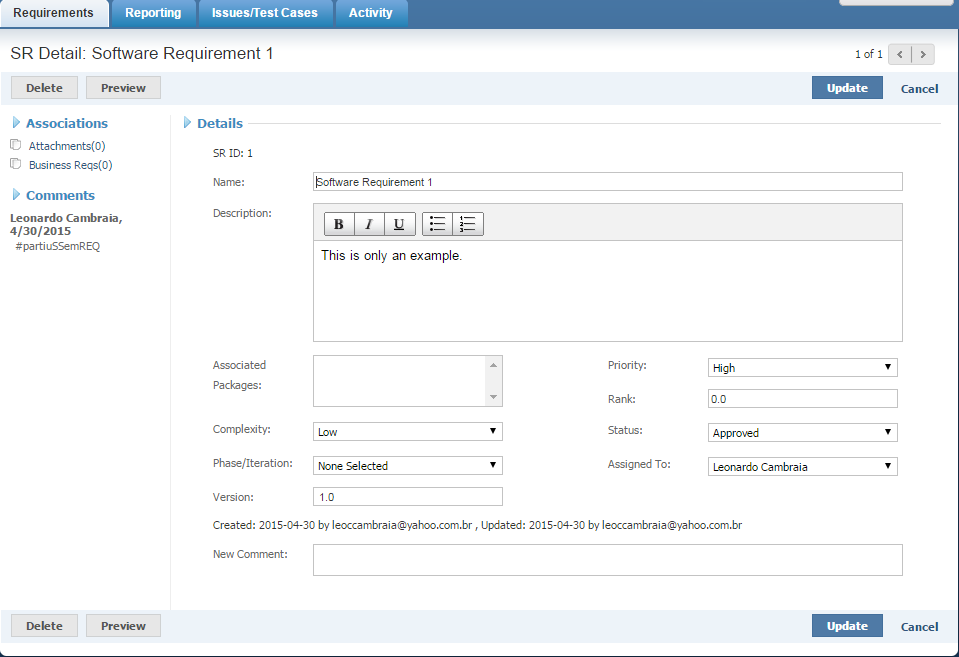
\includegraphics[scale=0.65]{editaveis/figuras/gatherspace_exemplo}
    \caption[Exemplo de um requisito na ferramenta GatherSpace.]
	{Exemplo de um requisito na ferramenta \textit{GatherSpace}.}
    \label{gatherspace_exemplo}
  \end{figure}
  
